\chapter{Integración compleja}
\label{chpt:integlacion_compleja}

Las funciones reales están definidas sobre conjuntos de números reales y con frecuencia se integran sobre intervalos. Las funciones complejas están definidas sobre conjuntos de puntos en el plano complejo y se integran sobre curvas. Antes de definir esta integral, es conveniente tener claro los conceptos de curvas paramétricas en el plano real y la integral de línea real (ver capítulo \ref{chpt:recordatorios}).

\section{Curvas paramétricas en el plano}

Si bien en la sección \ref{sec:1_curvas_y_regiones_en_el_plano_complejo} dimos una noción de lo que son las curvas y las regiones en el plano complejo para definir el dominio de una función compleja, en esta sección vamos a profundizar un poco sobre los conceptos de curvas cerradas, abiertas, suaves, entre otras propiedades que pueden tener. 

Una curva en el plano complejo es una función $\Gamma :[a,b]\to\mathbb{C}$, definida en un intervalo real $[a,b]$ y que toma valores complejos\footnote{$\Gamma$: letra griega Gamma mayúscula.}. Para cada número $t$ en $[a,b]$, $\Gamma(t)$ es un número complejo, o un punto en el plano. El lugar geométrico de tales puntos es la gráfica de la curva. Sin embargo, la curva es más que un lugar geométrico de puntos en el plano. $\Gamma$ tiene una orientación natural, que es la dirección en la que el punto $\Gamma(t)$ se mueve a lo largo de la gráfica conforme $t$ crece de $a$ a $b$. En este sentido, es natural referirse a $\Gamma(a)$ como el \textit{punto inicial} de la curva y a $\Gamma(b)$ como el \textit{punto final}.

Si $\Gamma(t)=x(t)+jy(t)$, entonces la gráfica de $\Gamma$ es el lugar geométrico de los puntos $(x(t),y(t))$ para $a\leqslant t\leqslant b$. El punto inicial de $\Gamma$ es $(x(a),y(a))$ y el punto final es $(x(b),y(b))$ y $(x(t),y(t))$ se mueve del punto inicial al punto final conforme varía $t$ de $a$ a $b$. Las funciones $x(t)$ e $y(t)$ son todas las \textit{funciones coordenadas} de $\Gamma$.

\begin{example}
  Sea $\Gamma (t) = 2t + jt^2$ para $0\leqslant t\leqslant 2$. Entonces:
  $$
  \Gamma (t)=x(t)+jy(t),
  $$
  donde $x(t)=2t$ y $y(t)=t^2$. La gráfica de esta curva es la parte de la parábola $y=(x/2)^2$, que se muestra en la figura \ref{fig:ejemplo_parabola_gamma}.
    \begin{figure}[ht]
    \centering
    \begin{tikzpicture}[scale=0.7,>=stealth]
      % Ejes y grid
      \draw[step=1cm,gray,loosely dotted] (-0.2,-0.2) grid (4.5,4.5);
      \draw[->] (-0.5,0) -- (4.5,0) node[right] {\footnotesize$x(t)$};
      \draw[->] (0,-0.5) -- (0,4.5) node[above] {\footnotesize$y(t)$};
      \node[below left] at (0,0) {\scriptsize0};
      \foreach \i in {1,...,4}
        {
          \node[below] at (\i,0) {\scriptsize\i}; 
          \node[left] at (0,\i) {\scriptsize\i}; 
        }
      % Curva parabólica 
      \begin{scope}[very thick,decoration={
        markings,
        mark=at position 0.5 with {\arrow{>}}}
        ] 
        \draw[red,>->,postaction={decorate}] (0,0) parabola (4,4) node[above right] {$\Gamma(t)$};
      \end{scope}
      \end{tikzpicture}
    \caption{Gráfica de la curva $\Gamma (t) = 2t + jt^2$, $0\leqslant t\leqslant 2$.}
    \label{fig:ejemplo_parabola_gamma}
  \end{figure}

  Conforme $t$ varía de $0$ a $2$, el punto $\Gamma (t)=(2t,t^2)$ se mueve a lo largo de esta gráfica del punto inicial $\Gamma(0)=(0,0)$ al punto final $\Gamma(2)=(4,4)$. Las flechas indican esta orientación.
\end{example}

\begin{example}
  Sea $\Gamma(t)=e^{jt}$ para $0\leqslant t \leqslant 3\pi$. Entonces $\Gamma(t)=\cos(t)+j\sin(t)=x(t)+jy(t)$, así
  \begin{equation*}
    x(t)=\cos(t),\qquad y(t)=\sin(t)
  \end{equation*}

    \begin{figure}[ht]
    \centering
    \begin{tikzpicture}[scale=1.5,>=stealth]
      % Ejes y grid
      \draw[step=0.5cm,gray,loosely dotted] (-1.9,-1.4) grid (1.9,1.4);
      \draw[->] (-2,0) -- (2,0) node[right] {\footnotesize$x(t)$};
      \draw[->] (0,-1.5) -- (0,1.5) node[above] {\footnotesize$y(t)$};
      % leyenda de números de ejes
      \node[below left] at (0,0) {\scriptsize0};
      % eje x
      \node[below] at (0.5,0) {\scriptsize$\frac{1}{2}$}; 
      \node[below right] at (1,0) {\scriptsize $\Gamma(0)=1$}; 
      \node[below] at (-0.5,0) {\scriptsize$-\frac{1}{2}$}; 
      \node[below left] at (-1,0) {\scriptsize $\Gamma(3\pi)=-1$}; 
      % eje y
      \node[left] at (0,0.5) {\scriptsize$\frac{1}{2}$}; 
      \node[above left] at (0,1) {\scriptsize 1}; 
      \node[left] at (0,-0.5) {\scriptsize$-\frac{1}{2}$}; 
      \node[below left] at (0,-1) {\scriptsize -1}; 

      \begin{scope}[very thick,decoration={
        markings,
        mark=at position 0.2 with {\arrow{>}},
        mark=at position 0.6 with {\arrow{>}},
        mark=at position 0.9 with {\arrow{>}},
      }] 
        \draw[red,postaction={decorate}] (0,0) circle (1);
      \end{scope}
      
      \coordinate (A) at (1,0);
      \coordinate (B) at (-1,0);
      \coordinate (C) at (45:1);
      \foreach \point in {A,B,C}
        \fill [black,opacity=.5] (\point) circle (2pt);
      \node[above right] at (C) {\scriptsize$\Gamma(t)=e^{jt}$};
    \end{tikzpicture}
    \caption{$\Gamma(t)=e^{jt}$ para $0\leqslant t\leqslant 3\pi$.}
    \label{fig:ejemplo_circunferencia_abierta_gamma}
  \end{figure}


  Como $x^2+y^2=1$, todo punto en esta curva está en el círculo unitario alrededor del origen. Sin embargo, el punto inicial de $\Gamma$ es $\Gamma(0)=1$ y el punto final es $\Gamma(3\pi)=e^{j3\pi}=-1$. Esta curva no es cerrada. Si esta fuera una pista de carreras, la carrera empezaría en el punto 1 de la figura \ref{fig:ejemplo_circunferencia_abierta_gamma} y terminaría en $-1$. Una pista de carreras circular no significa que los puntos de inicio y fin de la carrera sean el mismo. Esto no es evidente a partir sólo de la gráfica. $\Gamma$ está orientada positivamente, como lo indica la flecha.
  \label{ej:circunferencia_abierta}
\end{example}
\begin{example}
  Si se tomase el mismo caso que el ejemplo \ref{ej:circunferencia_abierta}, pero ahora el intervalo es $0\leqslant t \leqslant 4\pi$, resulta que ahora la curva si es cerrada, sin embargo $\Gamma(t)$ se mueve alrededor del círculo unitario dos veces conforme $t$ varía en el intervalo.
  \label{ej:circunferencia_cerrada_no_simple}
\end{example}

Una curva $\Gamma$ es \textit{simple} si $\Gamma(t_1)\neq \Gamma(t_2)$ siempre que $t_1\neq t_2$. Esto significa que el mismo punto nunca se repite en tiempos diferentes. Se hace una excepción para las curvas cerradas, que requieren que $\Gamma(a)=\Gamma(b)$. Si éste es el único punto en el cual $\Gamma(t_1)=\Gamma(t_2)$ con $t_1\neq t_2$, entonces $\Gamma$ es una \textit{curva cerrada simple}. La curva del ejemplo \ref{ej:circunferencia_cerrada_no_simple} es una curva cerrada, pero no simple. Si se define otra curva, igual a la del ejemplo \ref{ej:circunferencia_cerrada_no_simple} pero el intervalo es $0\leqslant t \leqslant 2\pi$, entonces $\Gamma$ es una curva cerrada simple.

Una curva $\Gamma:[a,b]\to \mathbb{C}$ es \textit{continua} si cada una de sus funciones coordenadas es continua en $[a,b]$. Si $x(t)$ y $y(t)$ son diferenciables en $[a,b]$, $\Gamma$ es una \textit{curva diferenciable}. Si $x'(t)$ y $y'(t)$ son continuas, y no valen cero para el mismo valor de $t$, $\Gamma$ es una \textit{curva suave}. Todas las curvas de los ejemplos anteriores son suaves.

En términos vectoriales, se puede escribir como $\Gamma(t)=x(t)\hat{\imath} + y(t)\hat{\jmath}$ como se ha visto en el capítulo \ref{chpt:recordatorios}. Si $\Gamma$ es diferenciable, y $x'(t)$ y $y'(t)$ no son cero, entonces $\Gamma'(t)=x'(t)\hat{\imath}+y'(t)\hat{\jmath}$ es el vector tangente a la curva en el punto $\Gamma(t)$ (figura \ref{fig:vector_tangente_a_una_curva}). Si $\Gamma$ es suave, entonces las derivadas $x'(t)$ y $y'(t)$ son continuas, así que el vector tangente es continuo (se puede encontrar un único $\Gamma'$ para cada punto de la curva).

\begin{figure}[ht]
  \centering
  \begin{subfigure}[b]{0.48\textwidth}
    \centering
    \begin{tikzpicture}[>=stealth]
      % Ejes
      \draw[->] (-1,0) -- (3,0) node[right] {\footnotesize$x$};
      \draw[->] (0,-0.5) -- (0,1.5) node[above] {\footnotesize$y$};

      \begin{scope}[very thick,decoration={
        markings,
        mark=at position 0.3 with {\arrow{>}},
        mark=at position 0.5 with {
          \coordinate (G) at (0,0);
          \draw[->,black,opacity=.7] (0,0) -- (1,0) node[right] {\footnotesize$\Gamma'(t)$}; 
        },
      }] 
        \draw[red,postaction={decorate}] (-0.9,-0.4) .. controls (0,1.2) and (0.9,1.4) .. (2.8,1);
      \end{scope}
      \fill [black,opacity=.5] (G) circle (2pt);
      \draw[->,very thick,black,opacity=.7] (0,0) -- (G) node[below right] {$\Gamma(t)$};
    \end{tikzpicture}
    \caption{Vector tangente a una curva.}
    \label{fig:vector_tangente_a_una_curva}
  \end{subfigure}
  \hfill
  \begin{subfigure}[b]{0.48\textwidth}
    \centering
    \begin{tikzpicture}[>=stealth]
      % Ejes
      \draw[->] (-1.5,0) -- (2.5,0) node[right] {\footnotesize$x$};
      \draw[->] (0,-0.5) -- (0,1.5) node[above] {\footnotesize$y$};

      \coordinate (A) at (-1.4,0.5);
      \coordinate (B) at (0.3,1);
      \begin{scope}[very thick,decoration={
        markings,
        mark=at position 0.3 with {\arrow{>}},
        mark=at position 0.5 with {
          \node[above] {\scriptsize$\Gamma_1$};
        },
      }] 
        \draw[red,postaction={decorate}] (A) .. controls (-0.9,0.9) and (-0.4,1.1) .. (B);
      \end{scope}
      \coordinate (C) at (0.6,0.2);
      \node[red,fill=white] at (0,0.6) {\scriptsize$\Gamma_2$};
      \begin{scope}[very thick,decoration={
        markings,
        mark=at position 0.5 with {\arrow{>}},
      }] 
        \draw[red,postaction={decorate}] (B) .. controls (0.35,0.5) .. (C);
      \end{scope}
      \coordinate (D) at (1.3,1.3);
      \begin{scope}[very thick,decoration={
        markings,
        mark=at position 0.5 with {\arrow{>}},
        mark=at position 0.6 with {
          \node[above=5pt] {\scriptsize$\Gamma_3$};
        }
      }] 
        \draw[red,postaction={decorate}] (C) .. controls (0.7,0.6) and (0.9,1) .. (D);
      \end{scope}
      \coordinate (E) at (2.4,-0.4);
      \begin{scope}[very thick,decoration={
        markings,
        mark=at position 0.4 with {\arrow{>}},
        mark=at position 0.5 with {
          \node[right] {\scriptsize$\Gamma_4$};
        }
      }] 
        \draw[red,postaction={decorate}] (D) .. controls (1.9,1.2) and (2,-0.4) .. (E);
      \end{scope}

      \foreach \i in {A,B,C,D,E} 
        \fill [gray] (\i) circle (2pt);
    \end{tikzpicture}
    \caption{La \textit{concatenación}.}
    \label{fig:curva_a_trozos}
  \end{subfigure}
\end{figure}


A veces se forma una curva $\Gamma$ juntando varias curvas $\Gamma_1,\dots, \Gamma_n$ en sucesión. Es importante que, el punto final de $\Gamma_{k-1}$ debe ser el mismo que el punto inicial de la siguiente curva $\Gamma_k$ para $k=1,\dots,n$ (figura \ref{fig:curva_a_trozos}). Una curva así se llama la \textit{concatenación} de $\Gamma_1,\dots,\Gamma_n$. Las curvas $\Gamma_k$ son las \textit{componentes} de esta concatenación. Si cada componente de una concatenación es suave, entonces es una curva \textbf{suave a trozos}. Tiene una tangente continua en cada punto, excepto quizá en los puntos de conexión entre curvas. Si la conexión es de manera suave (como sucede en la conexión entre $\Gamma_3$ y $\Gamma_4$ en la figura \ref{fig:curva_a_trozos}), la concatenación puede tener una tangente en cada uno de estos puntos y ella misma ser suave. En otras palabras, cuando la conexión entre dos curvas es suave, puede existir la derivada en la conexión, y ser tratada como una curva suave completa (y no suave a trozos).


\section{La integral compleja}

\begin{definition}
Sea $f$ una función compleja y $\Gamma:[a,b]\to\mathbb{C}$ una curva suave en el plano. Suponiendo que $f$ es continua en todos los puntos de $\Gamma$, entonces la integral de $f$ sobre $\Gamma$ se define como
$$
\int_\Gamma f(z)\,dz = \int_a^b f(\Gamma(t))\Gamma'(t)\,dt
$$
Como $z=\Gamma(t)$ en la curva, esta integral se escribe frecuentemente como
$$
\int_\Gamma f(z)\,dz = \int_a^b f(z(t))z'(t)\,dt
$$
Esta formulación tiene la ventaja de sugerir la manera que $\int_\Gamma f(z)dz$ es evaluada. Reemplazando $z$ con $z(t)$ en la curva y encontrando la expresión $dz=z'(t)dt$ sobre el intervalo $a\leqslant t\leqslant b$. 
\end{definition}


\section{Teorema de Cauchy}

El teorema de Cauchy (o integral de Cauchy) es considerado el teorema fundamental de la integración compleja. El enunciado del teorema usa implícitamente el teorema de la curva de Jordan, que establece que una curva continua, simple y cerrada en el plano separa al plano en dos conjuntos abiertos. Uno de estos conjuntos es no acotado y se llama el \textit{exterior}, y el otro es acotado y se llama el \textit{interior}. La curva misma no pertenece a ninguno de estos conjuntos, pero marca la frontera de ambos.

\begin{figure}[ht]
  \centering
  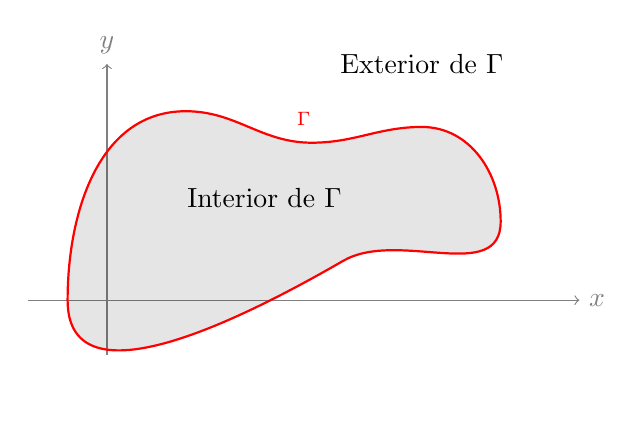
\begin{tikzpicture}
    \draw[->,gray] (-1,0) -- (6,0) node[right] {$x$};
    \draw[->,gray] (0,-0.7) -- (0,3) node[above] {$y$};

    \draw[thick,red,fill=black,fill opacity=0.1] (-0.5,0) to [out=90,in=180] (1,2.4)
    to [out=0,in=180] (2.6,2) 
    to [out=0,in=180] (4,2.2)
    to [out=0,in=90] (5,1)
    to [out=-90,in=30] (3,0.5)
    to [out=210,in=-90] (-0.5,0);
    \node[red] at (2.5,2.3) {\scriptsize$\Gamma$};

    \node at (2,1.3) {Interior de $\Gamma$};
    \node at (4,3) {Exterior de $\Gamma$};
  \end{tikzpicture}
  \caption{Teorema de la curva de Jordan.}
\end{figure}

A pesar de que esta conclusión puede parecer obvia para las curvas cerradas que se suelen dibujar, es difícil de probar debido a la generalidad de su enunciado. 

En la sección \ref{sec:1_curvas_y_regiones_en_el_plano_complejo} estuvimos analizando algunas regiones del plano complejo y sus propiedades. Esto lo hicimos para poder definir el dominio de una función compleja. Ahora vamos a profundizar algunos aspectos sobre las regiones del plano complejo para poder enunciar correctamente el teorema de Cauchy.

\begin{definition}[Trayectoria]
  Una trayectoria es una curva simple, suave a trozos. Una trayectoria pertenece a un conjunto $S$ si su gráfica está contenida dentro de $S$
\end{definition}

Algunas de las curvas paramétricas que hemos realizado anteriormente (como la figura \ref{fig:ejemplo_parabola_gamma}) son trayectorias en $\mathbb{C}$. Así, una trayectoria es una concatenación de curvas suaves que no se cruzan a sí mismas.

\begin{definition}[Conjunto conexo]
  Un conjunto $S$ de números complejos es conexo si, dados dos puntos cualesquiera de $z$ y $w$ en $S$, existe una trayectoria en $S$ que tiene a $z$ y a $w$ como puntos extremos.
\end{definition}

$S$ es conexo si es posible ir desde cualquier punto de $S$ a cualquier otro punto moviéndose a lo largo de alguna trayectoria totalmente contenida en $S$. Un disco abierto es conexo, así como también lo es un disco cerrado (ver sección \ref{sec:1_curvas_y_regiones_en_el_plano_complejo}).

\begin{definition}[Dominio]
  Como ya hemos visto, un conjunto de números complejos, abierto y conexo se llama dominio.
\end{definition}

\begin{definition}[Simplemente conexo]
  Un conjunto $S$ de números complejos es simplemente conexo si toda trayectoria cerrada en $S$ encierra únicamente puntos de $S$.
\end{definition}

Todo disco abierto es simplemente conexo. Si dibuja una trayectoria cerrada en un disco abierto, esta trayectoria cerrada encerará solamente puntos en el disco abierto. El anillo o corona de la figura \ref{fig:corona_complx} no es simplemente conexo. A pesar de ser conexo, se puede dibujar una trayectoria cerrada contenida en el anillo que encierra puntos que no pertenecen al anillo (son aquellos puntos excluidos por la frontera interna).

Ahora si, estamos listos para enunciar el teorema de Cauchy.

\subsection[Enunciado del teorema]{El teorema de Cauchy}

\begin{theorem}[Teorema de Cauchy]
  Sea $f$ diferenciable en un dominio simplemente conexo $G$. Sea $\Gamma$ una trayectoria cerrada en $G$. Entonces
  \[
    \oint_\Gamma f(z)dz=0
  \]
\end{theorem}


\section{Fórmula de la integral de Cauchy}

La consecuencia más importante del teorema de la integral de Cauchy es la fórmula de la integral de Cauchy. Esta fórmula es de utilidad para calcular integrales. Igualmente importante es su rol primordial en la demostración del sorprendente hecho de que las funciones analíticas tienen derivadas de todos los órdenes (capítulo \ref{chpt:residuos}: residuos), y por tanto pueden ser representadas mediante series de Taylor. 

\begin{figure}[ht]
  \centering
  \begin{tikzpicture}
    \draw[dashed,rotate=20] (0,0) ellipse (3 and 2);
    \node at (2.3,1) {$D$};
    \begin{scope}[thick,decoration={
        markings,
        mark=at position 0.5 with {
          \coordinate (G) at (0,0);
          \node[left] at (0,0) {\footnotesize$\Gamma$}; 
        },
        mark=at position 0.6 with {\arrow{>}},
      }]
      \draw[red,postaction={decorate}] (0,0) ellipse (1.5 and 0.9);
      \draw[fill] (0.3,0.2) circle (1pt) node[right] {\footnotesize$z_0$};
    \end{scope}
  \end{tikzpicture}
  \caption{Fórmula integral de Cauchy.}
  \label{fig:f_in_cauchy}
\end{figure}

\begin{theorem}\label{teo:formula_de_la_integral_de_cauchy}
  Sea $f(z)$ analítica en un dominio simplemente conexo $D$. Entonces para cualquier punto $z_0$ en $D$ y cualquier trayectoria simple cerrada $\Gamma$ en $D$ que contenga a $z_0$ (figura \ref{fig:f_in_cauchy}) se cumple 
  \begin{equation}
    \oint_\Gamma \frac{f(z)}{z-z_0}dz = j2\pi f(z_0)
    \label{eq:formula_de_la_integral_de_cauchy}
  \end{equation}
  donde la curva $\Gamma$ se recorre en sentido antihorario.
\end{theorem}

\begin{proof}
  Por adición y sustracción, $f(z)=f(z_0)+[f(z)-f(z_0)]$. Al sustituir esto en el miembro izquierdo de la ecuación \eqref{eq:formula_de_la_integral_de_cauchy} y sacando de la integral el factor constante $f(z_0)$, se obtiene
  \begin{equation}
    \oint_\Gamma \frac{f(z)}{z-z_0}dz = f(z_0)\oint_\Gamma \frac{1}{z-z_0}dz + \oint_\Gamma \frac{f(z)-f(z_0)}{z-z_0}dz
    \label{eq:demostracion_formula_integral_cauchy}
  \end{equation}
  Resolviendo el primer término del miembro derecho, vemos que $\Gamma$ es una curva paramétrica no conocida que encierra al punto $z_0$. Con ello, podemos aplicar el teorema de deformación \ref{teo:cauchy_doblemente_conexo} y podemos sustituir la curva $\Gamma$ por una circunferencia centrada en $z_0$ de radio $r$, tal que $r>0$ pero lo suficientemente pequeño como para estar dentro de $D$. De este modo se cumple la siguiente igualdad
  \begin{gather*}
    f(z_0)\oint_\Gamma \frac{1}{z-z_0}dz = f(z)\oint_\gamma \frac{1}{z-z_0}dz
  \end{gather*}
  Y la curva $\gamma$ puede parametrizarse fácilmente como $\gamma(t)=z_0+re^{jt}$ para $t\in[0\leqslant t \leqslant 2\pi]$. Entonces la integral queda
  \begin{gather*}
    \oint_\gamma \frac{1}{z-z_0}dz = j\int_0^{2\pi}\frac{re^{jt}}{\cancel{z_0}+re^{jt}-\cancel{z_0}}dt = j\int_0^{2\pi}1 dt = j2\pi
  \end{gather*}
  por tanto la ecuación \eqref{eq:demostracion_formula_integral_cauchy} puede escribirse como
  \begin{gather*}
    \oint_\Gamma \frac{f(z)}{z-z_0}dz = j2\pi f(z_0) + \oint_\Gamma \frac{f(z)-f(z_0)}{z-z_0}dz
  \end{gather*}
  Siguiendo el mismo razonamiento para la integral del segundo término con $\gamma(t)=z_0+re^{jt}$
  \begin{align*}
    \int_0^{2\pi} \frac{f(\gamma(t))-f(z_0)}{e^{jt}} ~ je^{jt} ~dt &= j\int_0^{2\pi} f(\gamma(t))-f(z_0) dt \\
                                                                   &= j\left( \int_0^{2\pi} f(z_0+re^{jt}) dt - f(z_0)\int_0^{2\pi}1 dt \right)
  \end{align*}
  Aquí como la curva $\gamma$ es una circunferencia de radio $r$, podemos decir que $r\to 0$ ($r$ tiende a cero) sin modificar el valor de la integral ya que se cumple el teorema \ref{teo:cauchy_doblemente_conexo} de la deformación. Véase que si $r\to 0$ entonces $f(z_0+re^{jt})\to f(z_0)$, por tanto, para un $r\to 0$ podemos escribir 
  $$
   \int_0^{2\pi} f(z_0+re^{jt}) dt - f(z_0)\int_0^{2\pi}1 dt = f(z_0) \int_0^{2\pi}1dt - f(z_0)\int_0^{2\pi}1dt
  $$
  siendo entonces cero el único valor posible para la integral
  $$
  \oint_\Gamma \frac{f(z)-f(z_0)}{z-z_0}dz = 0
  $$
  Quedando entonces la ecuación \eqref{eq:demostracion_formula_integral_cauchy} como 
  $$
    \oint_\Gamma \frac{f(z)}{z-z_0}dz = j2\pi f(z_0) + 0
  $$
  lo que se quería demostrar.
\end{proof}

\subsection{Ejemplos}

El teorema \ref{teo:formula_de_la_integral_de_cauchy} nos brinda una forma muy sencilla de calcular integrales. Para entender la aplicación veamos algunos ejemplos.

\begin{example}
  Evaluar 
  $$
  \oint_\Gamma \frac{e^{z^2}}{z-j}dz
  $$
  para cualquier trayectoria cerrada que no pase por $j$.

  Tenemos dos posibles casos.
  \begin{itemize}
    \item \textbf{Caso I}: $\Gamma$ no encierra a $j$. En este caso la integral es cero por el teorema de Cauchy.
    \item \textbf{Caso II}: $\Gamma$ encierra a $j$. Por la fórmula de la integral de Cauchy, con $z_0=j$, 
      $$
      \oint_\Gamma \frac{e^{z^2}}{z-j}dz = j2\pi f(j) = j\frac{2\pi}{e}
      $$
  \end{itemize}
\end{example}

\begin{example}
  Evaluar 
  $$
  \int_\Gamma \frac{e^{2z}\sin(z^2)}{z-2}dz
  $$
  sobre cualquier trayectoria que no pase por 2.

  Al igual que antes, tenemos dos casos posibles.
  \begin{itemize}
    \item \textbf{Caso I}: Si $\Gamma$ no encierra a 2, entonces $f(z)/(z-2)$ es analítica y la integral es cero.
    \item \textbf{Caso II}: Si $\Gamma$ encierra a 2, usamos la fórmula de la integral de Cauchy:
      $$
      \int_\Gamma \frac{e^{2z}\sin(z^2)}{z-2}dz = j2\pi f(2) = j2\pi e^4 \sin(4)
      $$
  \end{itemize}
\end{example}


\section{Derivadas de funciones analíticas}

Ahora se demostrará que una función compleja holomorfa (o diferenciable) en $D$ como se mencionó en la sección \ref{sec:definicion_de_analiticidad} también es analítica en $D$. Entonces dicha función tiene derivadas de todos los órdenes en todos los puntos de $D$.

Para funciones reales no hay un resultado como este. Una función real diferenciable puede no tener segunda derivada. Y si tiene segunda derivada, puede no tener una tercera, y así sucesivamente. En otras palabras, si una función real es diferenciable una vez, nada puede concluirse acerca de la existencia de la segunda derivada o derivadas superiores. Así, en este sentido las funciones analíticas complejas se comportan mucho más sencillamente que las funciones que las funciones reales.

\begin{theorem}[Derivadas de una función analítica]\label{teo:derivadas_de_todos_los_ordenes}
  Si $f(z)$ es analítica en un dominio $D$, entonces tiene derivadas de todos los órdenes en cada punto de $D$, las cuales entonces también son funciones analíticas en $D$.

  La derivada en un punto $z_0\in D$ se calcula como 
  \begin{equation}
    f^{(n)}(z_0) = \frac{n!}{j2\pi}\oint_\Gamma \frac{f(z)}{(z-z_0)^{n+1}}dz
  \end{equation}
  con $n=1,2,\dots$ y $\Gamma$ una curva simple cerrada que encierra únicamente puntos de $D$ y que contiene a $z_0$. Aquí se asume que el sentido de integración es antihorario.
\end{theorem}

\subsection{Demostración}

Primero, vamos a demostrar que se cumple para la primer derivada, siendo la expresión
$$
f'(z_0) = \frac{1}{j2\pi} \oint_\Gamma \frac{f(z)}{(z-z_0)^2}dz
$$

\begin{proof}
  Para demostrar que la derivada en un punto $z_0\in D$ puede escribirse usando el teorema \ref{teo:derivadas_de_todos_los_ordenes}, partimos de la definición de derivada 
  $$
  f'(z_0) = \lim_{\Delta z \to 0} \frac{f(z+\Delta z)-f(z)}{\Delta z}
  $$
  Usando la fórmula de la integral de Cauchy (ecuación \eqref{eq:formula_de_la_integral_de_cauchy}), podemos escribir las funciones del numerador como
  \begin{align*}
    f(z_0+\Delta z) &= \frac{1}{j2\pi}\oint_\Gamma \frac{f(z)}{z-(z_0+\Delta z)} dz \\ 
    f(z_0) &= \frac{1}{j2\pi} \oint_\Gamma \frac{f(z)}{z-z_0}dz
  \end{align*}
  Y, reemplazando estas expresiones en el límite y operando algebraicamente:
  \begin{align*}
    f'(z_0)=&\lim_{\Delta z \to 0} \frac{1}{j2\pi\Delta z} \left( \oint_\Gamma \frac{f(z)}{z-(z_0+\Delta z)}dz - \oint_\Gamma \frac{f(z)}{z-z_0}dz \right) \\ 
    =&\lim_{\Delta z \to 0} \frac{1}{j2\pi\Delta z} \left( \oint_\Gamma \frac{f(z)}{z-z_0-\Delta z} - \frac{f(z)}{z-z_0}dz \right) \\ 
    =&\lim_{\Delta z \to 0} \frac{1}{j2\pi\Delta z} \left( \oint_\Gamma \frac{f(z)(z-z_0)-f(z)(z-z_0-\Delta z)}{(z-z_0-\Delta z)(z-z_0)}dz \right) \\ 
    =&\lim_{\Delta z \to 0} \frac{1}{j2\pi\Delta z} \left( \oint_\Gamma \frac{\cancel{f(z)z}-\cancel{f(z)z_0}-\cancel{f(z)z}+\cancel{f(z)z_0}+f(z)\Delta z}{(z-z_0-\Delta z)(z-z_0)}dz \right) \\ 
    =&\lim_{\Delta z \to 0} \frac{\cancel{\Delta z}}{j2\pi\cancel{\Delta z}} \left( \oint_\Gamma \frac{f(z)}{(z-z_0-\Delta z)(z-z_0)}dz \right) \\  
    f'(z_0)=&\lim_{\Delta z \to 0} \frac{1}{j2\pi} \left( \oint_\Gamma \frac{f(z)}{(z-z_0-\Delta z)(z-z_0)}dz \right) 
  \end{align*}
  Y, en esta última expresión, puede verse claramente que si $\Delta z\to 0$, entonces la integral tiende a 
  $$
  \boxed{f'(z)=\frac{1}{j2\pi}\oint_\Gamma \frac{f(z)}{(z-z_0)^2}dz}
  $$
  quedando demostrado el teorema.
\end{proof}


## Resumen del Capítulo 2: Integración Compleja

### Introducción (chapters/2_integracion_fvc/main.tex)

Este capítulo introduce la integración de funciones complejas. A diferencia de las funciones reales que se integran sobre intervalos, las funciones complejas se integran sobre curvas en el plano complejo.

---

### 1. Curvas paramétricas en el plano (chapters/2_integracion_fvc/curvas.tex)

Esta sección define formalmente las curvas usadas en la integración compleja.

* **Curva Compleja:** Es una función $\Gamma$ que mapea un intervalo real $[a, b]$ a un conjunto de puntos en el plano complejo ($\Gamma :[a,b]\to\mathbb{C}$).
* **Orientación:** Las curvas tienen una dirección natural a medida que el parámetro $t$ crece de $a$ a $b$. Tienen un *punto inicial* $\Gamma(a)$ y un *punto final* $\Gamma(b)$.
* **Curva Simple:** Una curva que no se cruza a sí misma. Es decir, $\Gamma(t_1)\neq \Gamma(t_2)$ para valores distintos $t_1, t_2$.
* **Curva Cerrada Simple:** Una curva donde el punto inicial y final coinciden ($\Gamma(a)=\Gamma(b)$), pero este es el único punto donde la curva se toca a sí misma.
* **Curva Suave (Lisa):** Una curva $\Gamma(t) = x(t) + jy(t)$ donde las derivadas $x'(t)$ y $y'(t)$ son continuas y no son simultáneamente cero. El vector $\Gamma'(t)$ es el vector tangente a la curva.
* **Curva Suave a Trozos (Concatenación):** Una curva formada por la unión de varias curvas suaves conectadas en sucesión.

---

### 2. La integral compleja (chapters/2_integracion_fvc/integral.tex)

Esta sección define la integral compleja y sus propiedades fundamentales.

* **Definición de Integral Compleja:** La integral de una función $f(z)$ continua sobre una curva suave $\Gamma$ (parametrizada por $z(t)$ en $[a,b]$) se calcula como:
    $$
    \int_\Gamma f(z)\,dz = \int_a^b f(z(t))z'(t)\,dt
    $$
   
    Básicamente, se sustituye $z$ por $z(t)$ y $dz$ por $z'(t)dt$.
* **Integral sobre Curvas a Trozos:** Si la curva $\Gamma$ es una concatenación de curvas suaves ($\Gamma_1, \dots, \Gamma_n$), la integral total es la suma de las integrales sobre cada componente.
* **Propiedades:**
    * **Linealidad:** La integral de una suma de funciones (multiplicadas por constantes) es la suma de sus integrales.
    * **Inversión de la Orientación:** Recorrer la curva en sentido inverso cambia el signo de la integral.
* **Independencia de la Trayectoria (Teorema Fundamental):** Si $f(z)$ es una función analítica y continua en un dominio simplemente conexo $D$, y tiene una antiderivada $F(z)$ (tal que $F'(z)=f(z)$), la integral solo depende de los puntos extremos de la curva:
    $$
    \int_\Gamma f(z)dz = F(\Gamma(b))-F(\Gamma(a))
    $$
   
* **Consecuencia para Curvas Cerradas:** Si $f(z)$ es analítica (como en el punto anterior) y $\Gamma$ es una curva cerrada (los puntos inicial y final coinciden), la integral es cero:
    $$
    \oint_\Gamma f(z)dz = 0
    $$
   
* **Funciones no Analíticas:** Si la función $f(z)$ *no* es analítica, el resultado de la integral generalmente sí depende de la trayectoria tomada, no solo de los extremos.

---

### 3. Teorema de Cauchy (chapters/2_integracion_fvc/teo_de_cauchy.tex)

Esta sección presenta el teorema más importante de la integración compleja.

* **Conceptos Clave de Dominio:**
    * **Conjunto Conexo:** Un conjunto donde dos puntos cualesquiera pueden unirse mediante una trayectoria contenida totalmente en el conjunto.
    * **Conjunto Simplemente Conexo:** Un conjunto conexo que "no tiene agujeros". Formalmente, cualquier trayectoria cerrada simple dibujada dentro del conjunto encierra únicamente puntos que también pertenecen al conjunto. Un disco es simplemente conexo; una corona (anillo) no lo es.
* **Teorema de Cauchy (para Dominios Simplemente Conexos):**
    Si $f(z)$ es una función **analítica** en un dominio **simplemente conexo** $D$, entonces para *toda* trayectoria cerrada simple $\Gamma$ contenida en $D$, la integral es cero:
    $$
    \oint_\Gamma f(z)dz=0
    $$
   
* **Teorema de Deformación (para Dominios Múltiplemente Conexos):**
    Si $f(z)$ es analítica en un dominio *no* simplemente conexo (con agujeros), como una corona delimitada por una curva exterior $C_1$ y una curva interior $C_2$. La integral sobre la curva exterior es igual a la integral sobre la curva interior (asumiendo ambas en sentido antihorario):
    $$
    \oint_{C_1}f(z)dz = \oint_{C_2}f(z)dz
    $$
   
* **Principio de Deformación:** Este resultado permite "deformar" una trayectoria de integración $\Gamma_1$ a otra $\Gamma_2$ sin cambiar el valor de la integral, siempre y cuando la función $f(z)$ sea analítica en la región entre ambas curvas.
* **Generalización (Múltiples Agujeros):** Si una curva $C_1$ encierra varias curvas internas ($C_2, C_3, \dots$), la integral sobre $C_1$ es igual a la *suma* de las integrales sobre las curvas internas.

---

### 4. Fórmula de la integral de Cauchy (chapters/2_integracion_fvc/formula_int_cauchy.tex)

Esta sección describe una de las consecuencias más poderosas del Teorema de Cauchy, utilizada para calcular integrales que *no* son cero.

* **Fórmula de la Integral de Cauchy (Teorema):**
    Sea $f(z)$ analítica en un dominio simplemente conexo $D$. Sea $z_0$ un punto cualquiera dentro de $D$, y $\Gamma$ una trayectoria cerrada simple (en sentido antihorario) en $D$ que encierra a $z_0$. La fórmula establece:
    $$
    \oint_\Gamma \frac{f(z)}{z-z_0}dz = j2\pi f(z_0)
    $$
   
* **Importancia:** Esta fórmula es crucial. Permite calcular integrales de funciones con singularidades (como $1/(z-z_0)$) y es fundamental para demostrar que si una función es analítica, entonces sus derivadas de todos los órdenes también existen y son analíticas.

